%-----------------------------------------------------------------------------------------------------------------------------------------------------------------------------------------------
% Embasamento Teórico ou Fundamentação Teórica: revisão da literatura dos tópicos que sustentam a ciência e o conhecimento, relativos aos objetivos e aos métodos escolhidos para o desenvolvimento do trabalho.
% Itens como Considerações Iniciais e Finais não são obrigatórios, mas completam muito bem qualquer capítulo.
\chapter{Fundamentos Teóricos}
\label{Revisão Bibliográfica}


%-----------------------------------------------------------------------------------------------------------------------------------------------------------------------------------------------
A visão estéreo possibilita boa identificação de um espaço tridimensional, visto que sua estrutura permite a triangulação de pontos chaves, assim determinando o seu correto posicionamento. Deste modo, compreende-se o porquê deste sistema visual ser amplamente difundido na evolução humana e animal. Em visão computacional, deseja-se emular os sistemas de visão mais eficientes para identificação de objetos e reconhecimento de ambientes. Este processo pode ser realizado  computacionalmente, porém alguns conceitos como: Triangulação, Geometria Epipolar, Calibração e Retificação e Correspondência Estéreo. Estes conceitos encontram-se apresentados nas próximas seções abaixo.


%-----------------------------------------------------------------------------------------------------------------------------------------------------------------------------------------------
\section{Visão Estéreo - \textit{Stereo Imaging}}
\subsection{Triangulação - \textit{Triangulation}}

Idealmente, a triangulação de um Ponto P de coordenadas globais $(X,Y,Z)$ pode ser realizada caso tenha-se uma estrutura estéreo, cujas lentes não apresentem distorção e estejam perfeitamente alinhadas. Deste modo, matematicamente, é possível abstrair os sensores das câmeras como dois planos coplanares entre si. Nessas condições, tem-se que os eixos ópticos das câmeras são paralelos. O eixo óptico, também conhecido como raio principal, é a reta que intercepta o ponto de centro de projeção ${O}$ e o ponto principal da lente ${c}$. Assumindo que as câmeras sejam exatamente iguais e alinhadas, tem-se que os pontos focais da câmera esquerda e da câmera direita são iguais ${f_l = f_r}$ e os pontos principais ${c^{left}_x}$ e  ${c^{right}_x}$ apresentam as mesmas coordenadas \cite{Bradski2008}. A figura \ref{stereo_image_geometric_model} ilustra a representação do modelo idealizado de um sistema estéreo.

\begin{figure}[H]
 	\centering
 	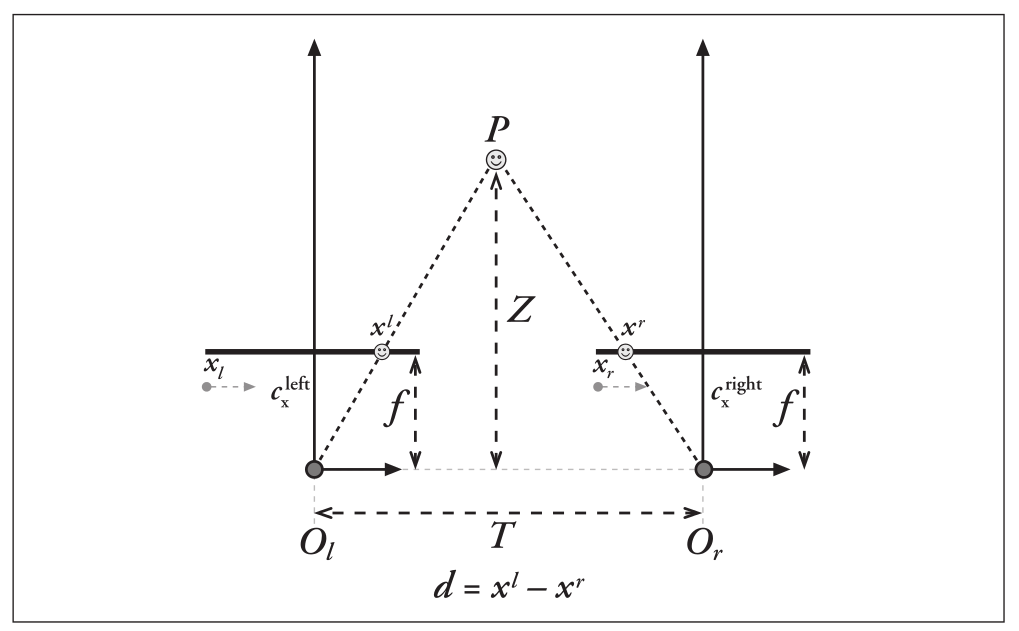
\includegraphics[scale=0.35]{./Resources/stereo_image_geometric_model.png}
 	\caption{Modelo Idealizado de um sistema de visão estéreo. Imagem retirada de \cite{Bradski2008}}
 	\label{stereo_image_geometric_model}
\end{figure}

A distância presente entre os pontos $x^l$ e $x^r$ é dada pela equação $d = x^l - x^r$, o valor de $d$ é comumente também de chamado de disparidade. Caso os pontos $x^l$ e $x^r$, a distância focal $f$, a distância entre os centros das câmeras $(T)$ (\textit{baseline}) sejam conhecidos é possível determinar a distância entre o Ponto P à base das câmeras $(Z)$. Por meio de semelhanças de triângulos, é possível estabelecer uma relação entre os triângulos $O_lPO_r$ e $x^lPx^r$, a qual está apresentada a seguir:
\begin{align*}
\frac{T - (x^l-x^r)}{Z-T} = \frac{T}{Z} \Rightarrow Z = \frac{fT}{(x^l-x^r)} = \frac{fT}{d}
\end{align*}


%-----------------------------------------------------------------------------------------------------------------------------------------------------------------------------------------------
\subsection{Geometria epipolar - \textit{Epipolar Geometry}}

Geometria epipolar corresponde à estrutura básica de um sistema estéreo, na qual leva em consideração os modelos \textit{pinhole} de ambas câmeras utilizadas e encontra-se ilustrada pela figura \ref{geometry_epipolar}. 

\begin{figure}[H]
 	\centering
 	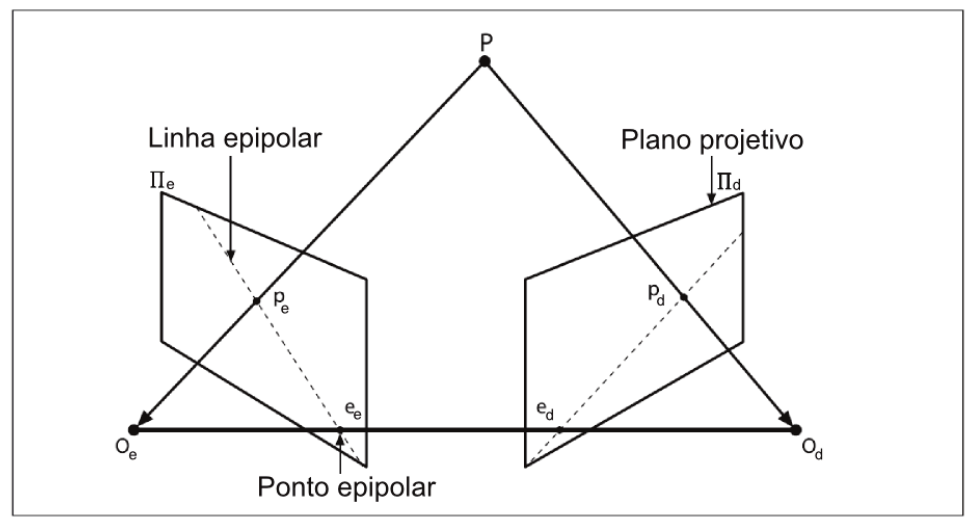
\includegraphics[scale=0.35]{./Resources/geometry_epipolar.png}
 	\caption{Geometria Epipolar. Imagem retirada de \cite{Mendes2012}}
 	\label{geometry_epipolar}
\end{figure}

Projeta-se o ponto P no centros de projeção $O^e$ e $O^d$, as linha que interligam o ponto P à esses centros interceptam os planos $\Pi_e$ e $\Pi_d$ nos pontos $p_e$ e $p_d$. Os pontos epipolares (\textit{epipoles}) $e_e$ e $e_d$ estão localizados nos pontos de intersecção da linha que interliga os centros de projeção e os planos projetivos. 

% Explicar Restrição epipolar
% Definição: Restrição Epipolar
% Pontos de correspondência devem estar em linhas epipolares conjugadas.

% A utilidade deste modelo está na chamada restrição epipolar. Suponha-se que, utilizando um
% sistema estéreo, pretende-se procurar na imagem da direita o ponto correspondente ao ponto p e ,
% projeção do ponto P na imagem da direita. A princípio, o ponto correspondente poderia estar
% em qualquer parte do plano projetivo da direita (Π d ). Nesse caso, seria necessário realizar
% uma busca bidimensional no plano projetivo Π d . Mas a “restrição epipolar” diz que o ponto
% correspondente ao ponto p e só pode estar na linha epipolar da direita. Como os valores de e e ,
% p e e e d são conhecidos, podemos então calcular a linha epipolar da direita e restringir a busca
% pelo ponto p d a esta linha. Isso reduz o escopo da busca de duas dimensões para apenas uma,
% economizando um possível gasto computacional ao realizar esta busca.
% Para fazer valer a “restrição epipolar” é preciso calibrar o sistema estéreo. O processo de
% calibração é descrito na Seção 2.1.5.
% 2.1.5


% We learned that we can find the image x of a 3D point X by tracing a line joining this 3D point
% with the camera's center. Conversely, the image point that we observe at position x can be
% located anywhere on this line in 3D space. This implies that if we want to find the corresponding
% point of a given image point in another image, we need to search along the projection of this line
% onto the second image plane. This imaginary line is called the epipolar line of point x. It defines
% a fundamental constraint that must satisfy two corresponding points, that is, the match of a
% given point must lie on the epipolar line of this point in the other view. The exact orientation of
% this epipolar line depends on the respective position of the two cameras. In fact, the position of
% the epipolar lines characterizes the geometry of a two-view system.
% Another observation that can be made from the geometry of this two-view system is that all
% of the epipolar lines pass through the same point. This point corresponds to the projection of
% one camera center onto the other camera. This special point is called an epipole.
% 
% $p'^TFp = 0$ 
% 
% This equation expresses the relation between two corresponding points and is known as the
% epipolar constraint


%-----------------------------------------------------------------------------------------------------------------------------------------------------------------------------------------------
%\section{Calibração \textit{Stereo Calibration}}
%\subsection{Parâmetros intrínsecos}

%\subsection{Parâmetros extrínsecos}

% Calibração
% Na realidade câmeras não são perfeitas, por conta do uso de lentes, a imagem formada possui
% distorções e seu centro ótico não é perfeitamente alinhado. Portanto é necessário um processo
% para estimar os parâmetros intrínsecos de cada câmera, isto é, a matriz M descrita na Seção
% 2.1.1 e o vetor D apresentado na Seção 2.1.2. No caso de um sistema estéreo, por conta de um
% alinhamento naturalmente imperfeito das câmeras, ainda se faz necessário estimar a matriz de
% rotação R e o vetor de translação T que relacionam as duas câmeras. As matrizes R e T são
% chamados de parâmetros extrínsecos e são ilustrados pela Figura 2.7.
% Os parâmetros extrínsecos são necessários para estimar os pontos epipolares, e assim fazer
% valer a “restrição epipolar”. Além disso, é possível alinhar as linhas epipolares horizontalmente,
% simplificando ainda mais a busca por pontos correspondentes. O processo de alinhar as imagens
% horizontalmente é chamado de retificação e é descrito na Seção 2.1.6.
% Existem vários métodos para estimar os parâmetros intrínsecos e extrínsecos (Zhang, 2008)
% de uma câmera, porém a descrição de tais métodos foge ao escopo desta dissertação. O método
% utilizado nesse projeto consiste na apresentação de um padrão conhecido para câmera estéreo
% (um tabuleiro de xadrez) onde é possível a identificação de pontos correspondentes entre o
% par de imagens estéreo. Isto possibilita ao método de calibração estimar todos os parâmetros
% necessários.Capítulo 2. Fundamentos Teóricos
% 13
% Figura 2.7: Por conta do alinhamento imperfeito presente em qualquer sistema estéreo é ne-
% cessário estimar as matrizes R e T que relacionam as câmeras (Bradski e Kaehler,
% 2008).
% 2.1.6


%----------------------------------------------------------------------------------------------------------------------------------------------------------------------------------------------
%\section{Retificação de Imagens  - \textit{Stereo Rectification}}

% Retificação
% O processo de retificação consiste em realizar uma transformação no par de imagens estéreo
% para alinhá-las horizontalmente, limitando assim a busca realizada pelo método estéreo, de
% duas, para uma dimensão. Utilizando as informações vindas da calibração os algoritmos de
% retificação objetivam minimizar a distorção a ser realizada nas imagens e ao mesmo tempo
% maximizar a área vista em comum pelas câmeras (Bradski e Kaehler, 2008). A Figura 2.8
% ilustra o resultado da retificação.
% 2.1.7


%-----------------------------------------------------------------------------------------------------------------------------------------------------------------------------------------------
\subsection{Correspondência Estéreo - \textit{Stereo Correspondence}}
Correspondência estéreo não é nada mais que a utilização de métodos estéreo, os quais são responsáveis pela procura de pontos homólogos nos pares de imagens estéreo. Como visto anteriormente, devido ao distanciamento das câmeras $(T)$ e ao distanciamento do objeto com relação às câmeras $(Z)$, o mesmo ponto apresenta diferentes posicionamento nos planos das câmeras $x^l$ e $x^r$. A figura \ref{homologous_points _stereo} ilustra um par de imagens estéreo (esquerda e direita), nas quais pixeis homólogos estão destacados. Os métodos estéreo utilizam da restrição epipolar o que reduzir o espaço de busca e de diferentes meios para encontrá-los. Mesmo com essa essa restrição e com a retificação das imagens, os métodos ainda assim apresenta um elevado custo computacional, além de que ainda estão sujeitos à encontrarem falsas correspondências \cite{Bradski2008}. 

\begin{figure}[H]
 	\centering
 	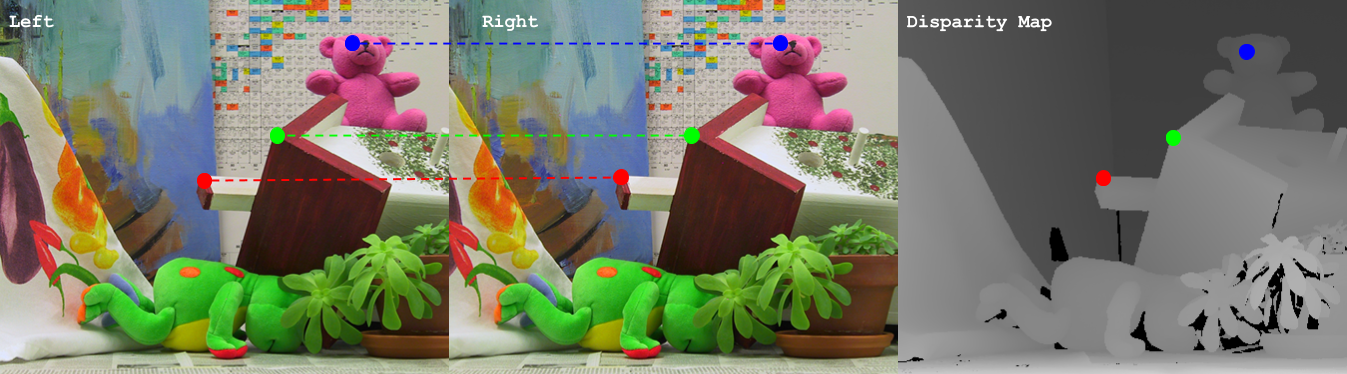
\includegraphics[scale=0.35]{./Resources/homologous_points_stereo.png}
 	\caption{Correspondência de pontos homólogos em um par de imagens estéreo}
 	\label{homologous_points _stereo}
\end{figure}

Abaixo, encontra-se apresentado um pequeno resumo de como são os operadores dos métodos estéreo utilizado neste trabalho.

\subsubsection{Método Estéreo - \textit{Block Matching} - BM}

\subsubsection{Método Estéreo Semi-global - \textit{Semi-global Block Matching} - SGBM}

\subsubsection{Método Estéreo Local com Aceleração de GPU - \textit{Block Matching with GPU Acceleration} - BMGPU}

% Remover Depois
% Pegar alguma das referências abaixo
% Métodos Estéreos
% Os métodos estéreos objetivam achar pontos homólogos em um par de imagens estéreo, a Figura
% 2.9 ilustra o problema. Mesmo em imagens retificadas o custo computacional de um método
% estéreo é alto, grande parte dos métodos existentes não são passíveis de serem usados em tempo
% real (Wang et. al., 2006b). Distorção projetiva, oclusão, descontinuidade e ambiguidade são
% alguns dos desafios que estes métodos tem de superar (Mattoccia, 2010). Por contar com tantos
% desafios, este tema é um dos mais investigados da área de visão computacional (Scharstein e
% Szeliski, 2002). Uma revisão geral sobre o tema é apresentada por Scharstein (1999) e Schars-
% tein e Szeliski (2002).


%-----------------------------------------------------------------------------------------------------------------------------------------------------------------------------------------------
\subsubsection{Mapa de disparidades - \textit{Disparity Map}}


%-----------------------------------------------------------------------------------------------------------------------------------------------------------------------------------------------
%\section{Projeção Tridimensional - \textit{3D Reprojection}}


%-----------------------------------------------------------------------------------------------------------------------------------------------------------------------------------------------
%\section{Reconhecimento de Objeto - \textit{Object Recognition}}
%\subsection{Segmentação - \textit{Image Segmentation}}

%\subsection{Identificação - \textit{Object Identification}}

%-----------------------------------------------------------------------------------------------------------------------------------------------------------------------------------------------
\subsection{Aplicações em Robótica}
\label{aplicacoes_robotica}
Nesta seção, serão apresentados alguns dos trabalhos que têm como principais sensores câmeras estéreo para a navegação autônoma em ambientes terrestre, aérea e subaquática.

Nos dias de hoje, as empresas automobilísticas vem participando de uma verdadeira corrida tecnológica para o desenvolvimento de automóveis totalmente autônomos e economicamente viáveis. As universidades não ficaram para trás e também apresentam pesquisas envolvendo desenvolvimento de algoritmos de controle e sensores, tornando essa corrida ainda mais acirrada. Os resultados apresentados são realmente promissores, o que concretizam cada vez mais essa realidade tida até então como distante. Na figura \ref{caminhao_autonomo} abaixo, é possível observar o projeto de caminhão autônomo desenvolvido pelo Laboratório de Robótica Móvel - LRM - ICMC/USP. O caminhão conta com diversos sensores, dentre eles câmeras estéreo, que identificam outros automóveis, pessoas e faixas de sinalização \cite{ShinzatoP}. 

\begin{figure}[H]
 	\centering
 	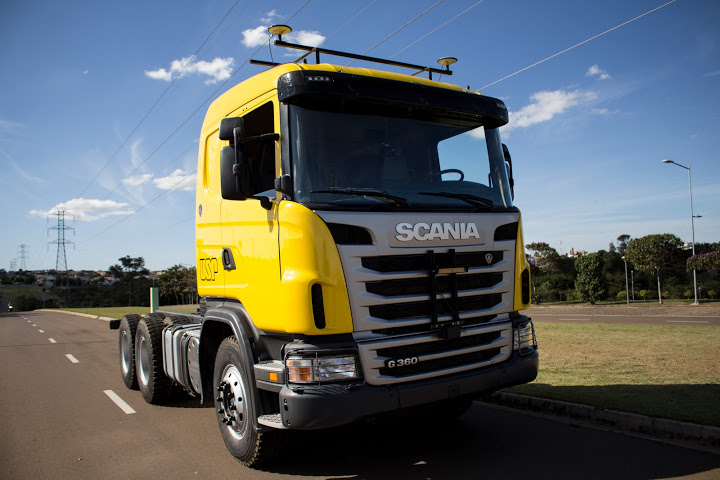
\includegraphics[scale=0.35]{./Resources/caminhao_autonomo.jpg}
 	\caption{Caminhão Autônomo desenvolvido pelo Laboratório de Robótica Móvel - LRM - ICMC/USP em parceria com a Scania}
 	\label{caminhao_autonomo}
\end{figure}

No caso de navegação autônoma para ambiente aéreo, o projeto utilizando \textit{Micro Air Vehicle} (MAVS) desenvolvido pelo \textit{Massachusetts Institute of Technology} (MIT) permite que estas pequenas aeronaves consigam navegar autonomamente e desviar de obstáculos voando a um velocidade de 30 mph (48 $km/h$). A figura \ref{mit_drones} abaixo apresenta o trabalho desenvolvido, o qual é um comparativo de desempenho de uma implementação em hardware utilizando \textit{Field-programmable gate array} (FPGA) e um processador ARM para processamento embarcado do método \textit{Semi-Global Block Matching} (SGBM) \cite{BarryMIT}.

\begin{figure}[H]
 	\centering
 	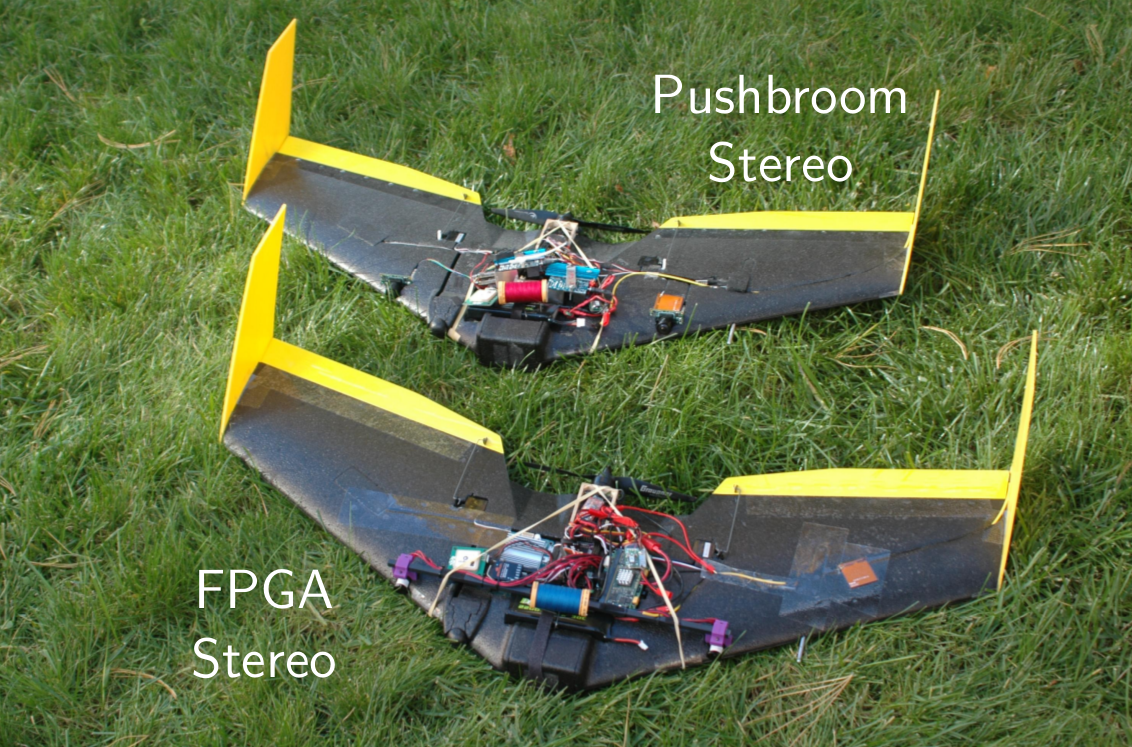
\includegraphics[scale=0.30]{./Resources/mit_drones.png}
 	\caption{Plataformas experimentais de aeronaves com o Sistema Estéreo - FPGA (frente) e o Sistema Estéreo - Pushbroom (trás). Câmaras são montados na parte dianteira das asas na mesma linha de base (34 cm) em ambas células.}
 	\label{mit_drones}
\end{figure}

No caso de navegação autônoma para ambiente subaquático, um exemplo de \textit{autonomous underwater vehicle} (AUV) é o projeto desenvolvido pela Universidade espanhola de Girona (veja figura \ref{G500}). O trabalho propõe a utilização do método de Mapeamento e Localização Simultânea (SLAM), juntamente com câmera estéreo, para o reconhecimento do ambiente, aprimorando assim o erro de rastreamento dos objetos \cite{Nagappa2013}.

\begin{figure}[H]
 	\centering
 	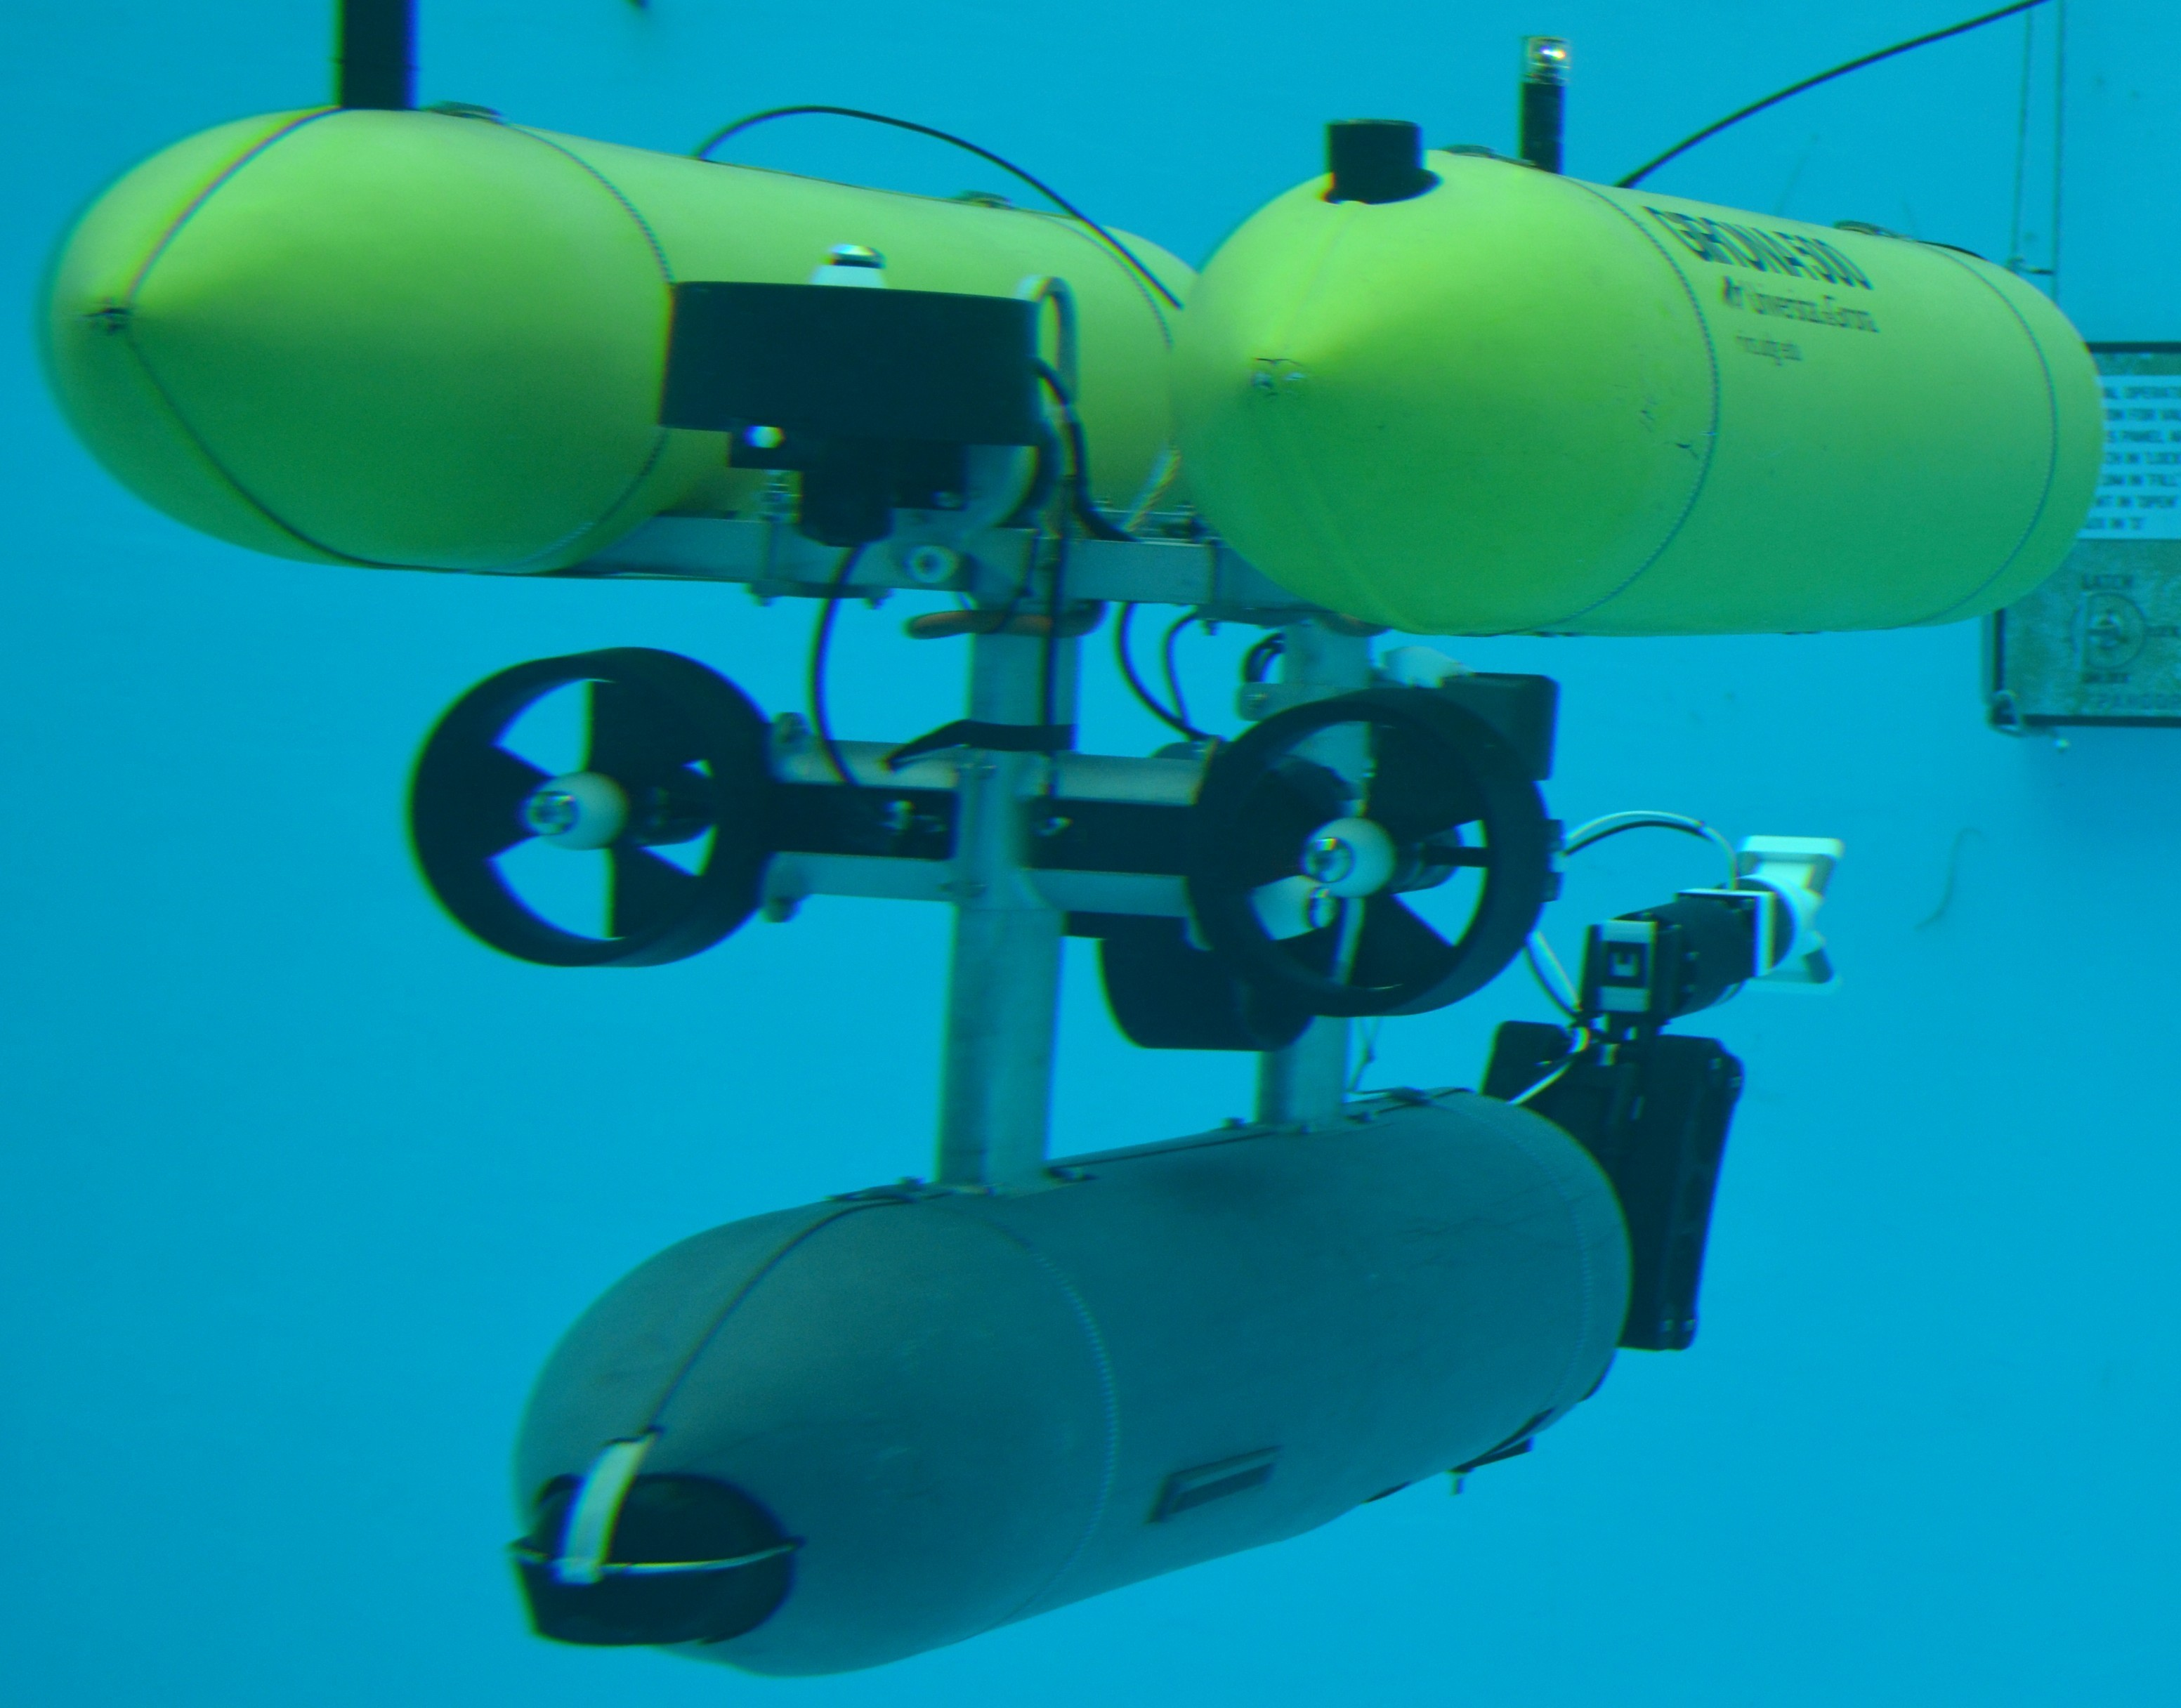
\includegraphics[scale=0.1]{./Resources/G500.jpg}
 	\caption{Veículo Submarino Autônomo - Girona 500}
 	\label{G500}
\end{figure}


%-----------------------------------------------------------------------------------------------------------------------------------------------------------------------------------------------